\documentclass[french,11pt,twoside]{VcCours}

\newenvironment{ApplicationDirecte}{\textbf{Application directe du cours :}

}{}
\newcommand{\dx}{\text{d}x}
\newcommand{\dt}{\text{d}t}
\DeclareMathOperator{\e}{e}
\newcommand{\Sum}[2]{\sum_{#1}^{#2}}
\newcommand{\Int}[2]{\int_{#1}^{#2}}

\renewcommand{\trou}[1]{{\color{white}#1}}
%\renewcommand{\trou}[1]{{\color{blue}#1}}

\begin{document}

\Titre{PSI}{Promotion 2021--2022}{Mathématiques}{Chapitre 6 : Suites et séries de fonctions}

\tableofcontents
\separationTitre

Dans tout le chapitre, $\mathbb{K}$ désigne $\mathbb{R}$ ou $\mathbb{C}$, $k$ un entier naturel non nul et $I$ est un intervalle de $\mathbb{R}$ contenant au moins deux points.


\section{Introduction} 

Pour tout $n \geq 0$, on considère la fonction $f_n$ définie pour tout $x \in I= [-1,1]$ par $f_n(x)=x^n$. Intéressons nous, pour tout $x \in [-1,1]$, à la convergence de la suite $(f_n(x))_{n \geq 0}$.


$\rhd$ \emph{Premier cas} : si $x=-1$.

% alors pour tout $n \geq 0$, $f_n(-1)=(-1)^n$ et donc $(f_n(-1))_{n \geq 0}$ diverge.
%
%\medskip

\vspace*{2.5cm}
$\rhd$ \emph{Deuxième cas} : si $x \in ]-1,1[$.
%
% alors pour tout $n \geq 0$, $f_n(x)=x^n$ et ainsi :
%$$ \lim_{n \rightarrow + \infty} f_n(x) = 0$$
%car $x \in ]-1,1[$.

\vspace*{2.5cm}


$\rhd$ \emph{Troisième cas} : si $x=1$.
%
% alors pour tout $n \geq 0$, $f_n(-1)=1$ et donc $(f_n(1))_{n \geq 0}$ converge vers $1$.
%
%\medskip
\vspace*{2.5cm}

Définissons la fonction \og limite \fg, notée $f$, de la suite $(f_n)_{n \geq 0}$ par :

\vspace*{2.5cm}
%$$ f(x) = \left\lbrace \begin{array}{ccl}
%0 & \hbox{ si } x \in ]-1,1] \\
%1 & \hbox{ si } x =1 \\
%\end{array}\right. ,$$

Plusieurs remarques sont alors naturelles : 

\begin{itemize}
\item Les fonctions $f_n$ sont définies sur $[-1,1]$ alors que $f$ n'est définie que sur $]-1,1]$.
\item Les fonctions $f_n$ sont continues sur $[-1,1]$ alors que $f$ n'est pas continue en $1$.
\end{itemize}

\medskip

\begin{center}
\emph{Quelques représentations graphiques}
\end{center}

\begin{center}
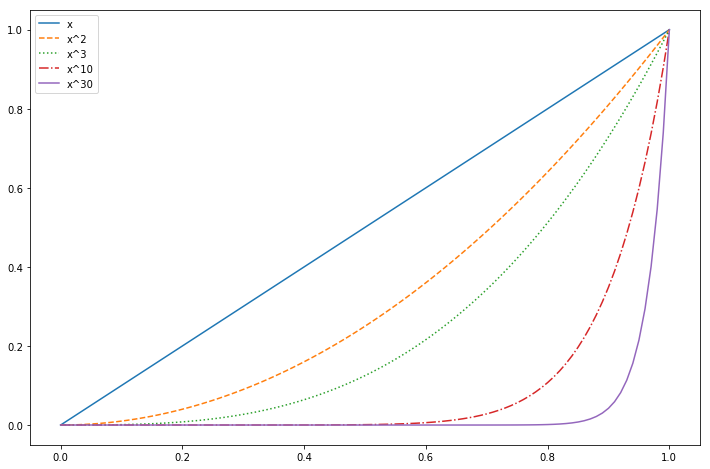
\includegraphics[scale=0.4]{Chap6-intro.png}
\end{center}

\medskip

Le but du chapitre est le suivant : 
si l'on considère une suite de fonctions $(f_n)_{n \geq 0}$ définies sur $I$ 
à valeurs dans $\mathbb{K}$, comment définir la convergence de cette suite ? 
Peut-on le faire de manière à conserver certaines propriétés (continuité ou 
dérivabilité par exemple) ? L'exemple précédent montre que la convergence \og{}
point par point \fg{} ne conserve pas la continuité\ldots

\medskip

On se posera ensuite les mêmes questions avec des séries de fonctions $\Sum{n \geq 0}{} f_n$ où $(f_n)_{n \geq 0}$ est une suite de fonctions définies sur $I$ à valeurs dans $\mathbb{K}$.


\section{Modes de convergence pour des suites de fonctions}

\subsection{Convergence simple}

\begin{Definition}{} Soit $(f_n)_{n \geq 0}$ une suite de fonctions définies sur $I$ à valeurs dans $\mathbb{K}$. On dit que $(f_n)_{n \geq 0}$ \emph{converge simplement} sur $I$ vers une fonction $f : I \rightarrow \mathbb{K}$ si :
$$ \phantom{\forall x \in I, \quad \lim_{n \rightarrow + \infty} f_n(x) = f(x)} $$
On note alors $f_n \xrightarrow[n \rightarrow + \infty]{\textrm{CVS}} f$.
\end{Definition}

\begin{Remarques}{}
\begin{itemize} 
\item La limite $f$ est unique quand elle existe car pour tout $x \in I$, $(f_n(x))_{n \geq 0}$ est une suite de scalaires. On dit que $f$ est la \emph{limite simple} de la suite $(f_n)_{n \geq 0}$ sur $I$.
\item On dit que $(f_n)_{n \geq 0}$ converge simplement sur $I$ s'il existe une fonction $f : I \rightarrow \mathbb{K}$ telle que $(f_n)_{n \geq 0}$ converge simplement vers $f$.
\item Généralement $f$ n'est pas donnée, on l'obtient en déterminant, pour tout $x \in I$, la limite de $(f_n(x))_{n \geq 0}$.
\end{itemize}
\end{Remarques}{}

\begin{Methode}{} Pour étudier la convergence simple de la suite $(f_n)_{n \geq 0}$, on commence par \emph{fixer} un élément $x$ de $I$ et on étudie la convergence de $(f_n(x))_{n \geq 0}$. Il est parfois nécessaire de distinguer des valeurs particulières pour $x$.
\end{Methode}

\medskip

\begin{Exemple}[\label{PremierEx}] Étudions la convergence simple sur $\mathbb{R}$ de la suite $(f_n)_{n \geq 1}$ définie par :
$$ \forall x \in \mathbb{R}, \quad f_n(x) = \sqrt{x^2 + \frac{1}{n}}$$

\newpage

%Soit $x \in \mathbb{R}$. On a :
%$$x^2 + \frac{1}{n} \underset{n \rightarrow + \infty}{\rightarrow} x^2 \geq 0$$
% puis par composition avec la fonction racine carrée qui est continue sur $\mathbb{R}_+$ :
%$$ f_n(x) \underset{n \rightarrow + \infty}{\rightarrow} \sqrt{x^2}= \vert x \vert $$
%Ainsi $(f_n)_{n \geq 0}$ converge simplement sur $\mathbb{R}$ vers la fonction valeur absolue.
\end{Exemple}

\begin{Exemple}[\label{Ex}] Étudions la convergence simple  sur $\mathbb{R}_+$ de la suite $(f_n)_{n \geq 0}$ définie par :
$$ \forall x \in \mathbb{R}_+, \quad f_n(x) = \frac{x^n}{x^n+1}$$

%Distinguons plusieurs cas :
%
%\begin{itemize}
%\item Si $x \in [0,1[$, on a $f_n(x) = \dfrac{x^n}{x^n+1} \underset{n \rightarrow + \infty}{\rightarrow} 0$.
%\item Si $x=1$, on a $f_n(1) = \dfrac{1}{2} \underset{n \rightarrow + \infty}{\rightarrow} \dfrac{1}{2} \cdot$
%\item Si $x \in ]1, + \infty[$, on a $f_n(x) = \dfrac{x^n}{x^n+1} = \dfrac{1}{1+ \frac{1}{x^n}} \underset{n \rightarrow + \infty}{\rightarrow} 1.$
%\end{itemize}
%
%\medskip
%
%Ainsi $f_n \xrightarrow[n \rightarrow + \infty]{\textrm{CVS}} f$ où $f : \mathbb{R}_+ \rightarrow \mathbb{R}$ est définie par :
%
%$$ f(x) = \left\lbrace \begin{array}{ccl}
%0 & \hbox{ si } x \in [0,1[ \\[0.1cm]
%\dfrac{1}{2} & \hbox{ si } x = 1 \\[0.3cm] 
%1 & \hbox{ si } x> 1 \\
%\end{array}\right.$$

\vspace*{8cm}

\end{Exemple}

\begin{Remarque}{} La convergence simple est donc une convergence \emph{ponctuelle} : on fixe $x \in I$ avant de passer à la limite. Cette convergence n'est pas satisfaisante en général, par exemple :

\begin{itemize}
\item L'exemple~\ref{Ex} et l'introduction montrent que la limite simple n'est pas nécessairement continue sur $I$ même si les fonctions $f_n$ le sont.
\item L'exemple~\ref{PremierEx} montre que même si la continuité est conservée pour la limite simple, ce n'est pas forcément le cas de la dérivabilité (dérivabilité en $0$ dans ce cas).
\end{itemize}
\end{Remarque}

\begin{ApplicationDirecte} Étudier la convergence simple sur $[0,1]$ de la suite $(f_n)_{n \geq 0}$ définie par :
$$ \forall x \in [0,1], \quad f_n(x) = n x^n(1-x)$$
\end{ApplicationDirecte}
\subsection{Convergence uniforme}

\begin{Definition}{} Soit $(f_n)_{n \geq 0}$ une suite de fonctions définies sur $I$ à valeurs dans $\mathbb{K}$. On dit que $(f_n)_{n \geq 0}$ \emph{converge uniformément} sur $I$ vers une fonction $f : I \rightarrow \mathbb{K}$ si : 
$$\phantom{\forall \varepsilon >0, \, \exists N \in \mathbb{N}, \, \forall n \geq N, \, \forall x \in I, \, \vert f_n(x)-f(x) \vert \leq \varepsilon}$$
On note dans ce cas : $f_n \xrightarrow[n \rightarrow + \infty]{\textrm{CVU}} f$.
\end{Definition}

%
%\begin{itemize}
%\item A partir d'un certain rang, les fonctions $f_n-f$ sont bornées sur $I$.
%\item $\sup_{x \in I} \vert f_n(x) - f(x) \vert \underset{n \rightarrow + \infty}{\rightarrow} 0$.
%\end{itemize}
%\end{Definition}


\begin{Remarque}{} 
%La deuxième condition précédente est équivalente à :
%$$ \forall \varepsilon >0, \, \exists N \in \mathbb{N}, \, \forall n \geq N, \, \forall x \in I, \, \vert f_n(x)-f(x) \vert \leq \varepsilon$$
%ou encore :
%$$\forall \varepsilon >0, \, \exists N \in \mathbb{N}, \, \forall n \geq N, \,  \sup_{x \in I} \vert f_n(x)-f(x) \vert \leq \varepsilon$$
La définition de convergence simple de $(f_n)_{n \geq 0}$ vers $f$ est équivalente à :
$$ \forall x \in I, \,  \forall \varepsilon >0, \, \exists N \in \mathbb{N}, \, \forall n \geq N,  \, \vert f_n(x)-f(x) \vert \leq \varepsilon$$
L'échange de quantificateur est ici extrêmement important : dans le cas de la convergence simple, le rang $N$ dépend du $x$ alors que dans le cas de la convergence uniforme, ce rang $N$ ne dépend pas de $x$ : la \og vitesse \fg{} de convergence est uniforme.
\end{Remarque}

\begin{Proposition}{}  Si une suite $(f_n)_{n \geq 0}$ converge uniformément vers une fonction $f$ sur un intervalle $I$ alors elle converge simplement vers $f$ sur $I$. Ainsi, $f$ est unique et est appelée la \emph{limite uniforme} de $(f_n)_{n \geq 0}$.
\end{Proposition}
\begin{Demonstration}{}

\vspace*{8cm}
\end{Demonstration}


\begin{Remarque}{} On dit que $(f_n)_{n \geq 0}$ converge uniformément sur $I$ s'il existe une fonction $f : I \rightarrow \mathbb{K}$ telle que $(f_n)_{n \geq 0}$ converge uniformément vers $f$ sur $I$. Cette définition est peu utilisée car dans la pratique, on commence par étudier la convergence simple et on connaît alors le candidat $f$ pour être la limite uniforme.
\end{Remarque}

\medskip

La définition de convergence uniforme n'étant pas très maniable, on introduit une nouvelle notion permettant de mieux étudier la convergence uniforme.

\subsection{Convergence uniforme et norme infini}
%
%\begin{Methode}{} On commence généralement par étudier la convergence simple de la suite de fonctions pour déterminer la fonction qui est potentiellement la limite uniforme.
%\end{Methode}
%
%\begin{Exemple} Considérons la suite de fonctions de l'introduction : pour tout $n \geq 0$, on considère la fonction $f_n$ définie pour tout $x \in I= [-1,1]$ par $f_n(x)=x^n$. On sait que $(f_n)_{n \geq 0}$ converge simplement sur $]-1,1]$ vers la fonction $f$ définie par :
%$$ f(x) = \left\lbrace \begin{array}{ccl}
%0 & \hbox{ si } x \in ]-1,1] \\
%1 & \hbox{ si } x =1 \\
%\end{array}\right. $$
%Étudions la convergence uniforme de $(f_n)_{n \geq 0}$ vers $f$ sur $]-1,1[$ :
%
%\begin{itemize}
%\item Pour tout $n \geq 0$, $f_n$ est continue sur $]-1,1]$ et la fonction $f$ est bornée donc les fonctions $f_n-f$ sont bornées.
%\item $\phantom{test}$
%Pour tout $n \geq 0$, on a :
%\begin{align*}
%\sup_{x \in ]-1,1]} \vert f_n(x) - f(x) \vert  & = \sup_{x \in ]-1,1[} \vert f_n(x) - f(x) \vert \quad \hbox{ car } f_n(1)=1=f(1) \\
%& = \sup_{x \in ]-1,1[} \vert x^n \vert  \\
%& = \sup_{x \in ]-1,1[} \vert x \vert^n   \\
%& = \sup_{x \in [0,1[} \vert x \vert^n   \quad \hbox{ par parité de } x \mapsto \vert x \vert \\
%& =  \sup_{x \in [0,1[} x^n \\
%\end{align*}
%Or la fonction $x \mapsto x^n$ est croissante sur $[0,1[$ donc :
%$$ \sup_{x \in [0,1[} x^n = \lim_{x \rightarrow 1^{-}} x^n = 1 \neq 0$$
%Ainsi $(f_n)_{n \geq 0}$ ne converge pas uniformément vers $f$ sur $]-1,1]$.

%\vspace*{7cm}
%\end{itemize}

%\end{Exemple}

\begin{Definition}{} Si une fonction $f$ est bornée sur un intervalle $I$ et à valeurs dans $\mathbb{K}$, on définit alors la \emph{norme infini} (ou norme de la \emph{convergence uniforme}) de $f$ et on note $\Vert f \Vert_{\infty}$ le réel positif défini par :
$$ \phantom{\Vert f \Vert_{\infty} = \sup_{x \in I} \vert f(x) \vert} $$
\end{Definition}

\begin{Remarques}{}
\begin{itemize} 
\item Si $f$ est bornée sur $I$, $\Vert f \Vert_{\infty}$ est bien défini car l'ensemble 
$$ \lbrace \vert f(x) \vert \, \vert \, x \in I \rbrace$$
est un sous-ensemble de $\mathbb{R}$ non vide et majorée donc admet une borne supérieure. Remarquons que si $f$ est continue sur le segment $I= [a,b]$ où $a$, $b$ sont deux réels tels que $a<b$ alors la borne supérieure est un maximum.
\item On note parfois $\Vert f \Vert_{I,\infty}$ si l'on souhaite préciser l'intervalle.
\end{itemize}
\end{Remarques}{} 

\begin{Theoreme}{} Soit $\mathcal{B}(I,\mathbb{K})$ l'ensemble des fonctions bornées sur $I$ à valeurs dans $\mathbb{K}$. Alors l'application :
$$ \begin{array}{ccccl}
\Vert \cdot \Vert & : & \mathcal{B}(I, \mathbb{K}) & \rightarrow & \mathbb{R}_+ \\
& & f & \mapsto & \Vert f \Vert_{\infty} \\
\end{array}$$
est ce que l'on appelle une \emph{norme} sur $\mathcal{B}(I,\mathbb{K})$, c'est-à-dire qu'elle vérifie les propriétés suivantes : 
\begin{enumerate}
\item Pour tout $f \in \mathcal{B}(I,\mathbb{K})$, $\Vert f \Vert_{\infty} = 0 \Longrightarrow f= \tilde{\theta}$ (\emph{séparation}).
\item Pour tout $f  \in \mathcal{B}(I,\mathbb{K})$ et tout $\lambda \in \mathbb{K}$, $\Vert \lambda f \Vert_{\infty} = \vert \lambda \vert \Vert f \Vert_{\infty}$ (\emph{homogénéité}).
\item Pour tout $(f,g) \in \mathcal{B}(I,\mathbb{K})^2$, $\Vert f+g \Vert_{\infty} \leq \Vert f\Vert_{\infty} + \Vert g \Vert_{\infty}$ (\emph{inégalité triangulaire}).
\end{enumerate}
\end{Theoreme}
\begin{Demonstration}{}

\vspace*{10cm}

\newpage

$\phantom{test}$

\vspace*{5cm}
\end{Demonstration}

\begin{Proposition}{}  Soit $(f_n)_{n \geq 0}$ une suite de fonctions définies sur $I$ à valeurs dans $\mathbb{K}$. Alors $(f_n)_{n \geq 0}$ converge uniformément vers une fonction $f : I \rightarrow \mathbb{K}$ si et seulement si les deux conditions suivantes sont vérifiées :  

\begin{itemize}
\item A partir d'un certain rang, les fonctions $f_n-f$ sont bornées sur $I$.
\item $\lim_{n \rightarrow + \infty} \Vert f_n - f  \Vert_{\infty} =0$.
\end{itemize}
\end{Proposition}

\begin{Demonstration}{} Conséquence directe de la définition de convergence uniforme.
%
%\vspace*{4cm}
\end{Demonstration}

\medskip

\begin{Exemple} Considérons la suite de fonctions de l'introduction : pour tout $n \geq 0$, on considère la fonction $f_n$ définie pour tout $x \in [-1,1]$ par $f_n(x)=x^n$. On sait que $(f_n)_{n \geq 0}$ converge simplement sur $]-1,1]$ vers la fonction $f$ définie par :
$$ f(x) = \left\lbrace \begin{array}{ccl}
0 & \hbox{ si } x \in ]-1,1] \\
1 & \hbox{ si } x =1 \\
\end{array}\right. $$
Étudions la convergence uniforme de $(f_n)_{n \geq 0}$ vers $f$ sur $]-1,1]$ :

\vspace*{7cm}

\vspace*{\stretch{1}}
\end{Exemple}

%
%
%\begin{Proposition}{} Soit $(f_n)_{n \geq 0}$ une suite de fonctions définies sur $I$ à valeurs dans $\mathbb{K}$. La suite $(f_n)_{n \geq 0}$ \emph{converge uniformément} vers une fonction $f : I \rightarrow \mathbb{K}$ si et seulement s'il existe une suite réelle $(a_n)_{n \geq 0}$ telles que les deux conditions suivantes soient vérifiées :
%
%\begin{itemize}
%\item A partir d'un certain rang, $\sup_{x \in I} \vert f_n(x)-f(x) \vert \leq a_n$.
%\item $\lim_{n \rightarrow + \infty} a_n = 0$.
%\end{itemize}
%\end{Proposition} 
%
%\begin{Remarque}{} $\sup_{x \in I} \vert f_n(x)-f(x) \vert = \Vert f_n -f \Vert_{ \infty}$.
%\end{Remarque}
%
%\begin{Demonstration}{} On raisonne par double implications.
%
%\medskip
%
%$\rhd$ Supposons que $(f_n)_{n \geq 0}$ converge uniformément vers $f$. A partir d'un certain rang $N$, les fonctions $f_n-f$ sont bornées et on pose dans ce cas :
%$$ a_n = \sup_{x \in I} \vert f_n(x)-f(x) \vert$$
%On pose $a_n=0$ pour tout $n \in \iii{0}{N}$. Par définition de la convergence uniforme, on a alors bien :
%$$ \lim_{n \rightarrow + \infty} a_n = 0$$
%
%\medskip
%
%$\rhd$ Supposons l'existence d'une une suite réelle $(a_n)_{n \geq 0}$, convergeant vers $0
%$, vérifiant à partir d'un certain rang, 
%$$ 0 \leq \sup_{x \in I} \vert f_n(x)-f(x) \vert \leq a_n$$
%Ainsi les fonctions $f_n-f$ sont bornées à partir de ce rang et par théorème d'encadrement, $\left(\sup_{x \in I} \vert f_n(x)-f(x) \vert \right)_{n \geq 0}$ est convergente et sa limite est $0$. Par passage aux quantificateurs, on obtient le résultat.
%\end{Demonstration}

\begin{Methode}{} Pour étudier la convergence uniforme d'une suite de fonctions $(f_n)_{n \geq 0}$  sur un intervalle $I$, on peut procéder de la manière suivante :

\begin{enumerate}
\item On étudie la convergence simple pour obtenir la limite simple (si elle existe) $f$.
\item On essaie de déterminer une suite $(a_n)_{n \geq 0}$ tendant vers $0$ telle qu'à partir d'un certain rang,
$$ \forall x \in I, \, \vert f_n(x)-f(x) \vert \leq a_n$$
ce qui est équivalent à :
$$ \Vert f_n - f \Vert_{\infty} \leq a_n$$
Dans ce cas, par théorème d'encadrement, on obtient que $(f_n)_{n \geq 0}$ converge uniformément vers $f$ sur $I$. \emph{Attention} : Le point important est de majorer avec un \emph{terme ne dépendant pas de $x$}.
\item S'il semble compliqué de majorer, on peut étudier les fonctions $x \mapsto f_n(x)-f(x)$ (dérivabilité, variations) afin de déterminer $\sup_{x \in I} \vert f_n(x)-f(x) \vert$ : la convergence est uniforme vers $f$ si cette expression tend vers $0$ quand $n$ tend vers $+ \infty$ (et ne converge pas uniformément sinon). 
\end{enumerate}
\end{Methode}

\begin{Exemple} 
On pose pour tout $n \geq 0$ et tout $x \in \mathbb{R}_+$, $f_n(x)= nx^2 e^{-nx}$. 
Étudions la convergence uniforme de $(f_n)_{n \geq 0}$ sur $\mathbb{R}_+$. 

\medskip

$\rhd$ Commençons par étudier la convergence simple sur $\mathbb{R}_+$.

%\begin{itemize}
%\item Si $x=0$, on a : $f_n(x) = 0 \underset{n \rightarrow + \infty}{\rightarrow} 0$.
%\item Si $x>0$, on a par théorème de croissances comparées : $f_n(x)= nx^2 e^{-nx} \underset{n \rightarrow + \infty}{\rightarrow} 0$.
%\end{itemize}
%Finalement, $f_n \xrightarrow[n \rightarrow + \infty]{\textrm{CVS}} f$ sur $\mathbb{R}_+$ où $f$ est la fonction nulle sur $\mathbb{R}_+$.
%
%\medskip

\vspace*{5cm}

$\rhd$ Étudions la convergence uniforme sur $\mathbb{R}_+$.

\vspace*{\stretch{1}}
% Pour tout $n \geq 0$, $f_n$ est dérivable sur $\mathbb{R}_+$ et l'on a :
% $$ \forall x \in \mathbb{R}_+, \quad f_n'(x) = n x e^{-nx}( 2-nx)$$
% Ainsi $f_n$ est croissante sur $[0, \frac{2}{n}]$ puis décroissante sur $[\frac{2}{n}, + \infty[$ et ainsi (en remarquant que $f_n$ est positive) : 
% $$ \sup_{x \in \mathbb{R}_+} \vert f_n(x) \vert = \sup_{x \in \mathbb{R}_+}  f_n(x)  = f_n \left( \frac{2}{n} \right) = \frac{4}{n} e^{-2}$$
% Or $\dfrac{4}{n} e^{-2} \underset{n \rightarrow + \infty}{\rightarrow} 0$ donc $f_n \xrightarrow[n \rightarrow + \infty]{\textrm{CVU}} f$ sur $\mathbb{R}_+$.
\end{Exemple}

\newpage

\begin{Remarque}{} Si $(f_n)_{n \geq 0}$ converge uniformément vers une fonction $f$ sur un intervalle $I$ alors pour tout suite $(x_n)_{n \geq 0}$ d'éléments de $I$, on a :
$$ \forall n \geq 0, \quad 0 \leq \vert f_n(x_n)-f(x_n) \vert \leq \sup_{x \in I} \vert f_n(x)- f(x) \vert$$
Par théorème d'encadrement, on montre alors que 
$$f_n(x_n)-f(x_n) \underset{n \rightarrow + \infty}{\longrightarrow} 0$$
Ainsi, si l'on trouve une suite $(x_n)_{n \geq 0}$ d'éléments de $I$ ne vérifiant pas cette condition, la suite $(f_n)_{n \geq 0}$ ne converge pas uniformément vers $f$ sur $I$.
\end{Remarque}

\medskip

\begin{Exemple} On pose pour tout $n \geq 0$ et tout $x \in \mathbb{R}_+$, $f_n(x)= e^{-nx} \sin(nx)$.

\begin{enumerate}
\item Étudions la convergence simple de $(f_n)_{n \geq 0}$ sur $\mathbb{R}_+$. 
%
%\begin{itemize}
%\item Si $x=0$, on a : $f_n(x) = 0 \underset{n \rightarrow + \infty}{\rightarrow} 0$.
%\item Si $x>0$, on a pour tout $n \geq 0$,
%$$ 0 \leq \vert f_n(x) \vert \leq e^{-nx}$$
%Or $e^{-nx} \underset{n \rightarrow + \infty}{\rightarrow} 0$ donc par théorème d'encadrement $(f_n(x))_{n \geq 0}$ est convergente et sa limite est nulle.
%\end{itemize}
%Finalement, $f_n \xrightarrow[n \rightarrow + \infty]{\textrm{CVS}} f$ sur $\mathbb{R}_+$ où $f$ est la fonction nulle sur $\mathbb{R}_+$.

\vspace*{7cm}
\item Étudions la convergence uniforme $(f_n)_{n \geq 0}$ sur $[a, + \infty[$ où $a>0$. 

\vspace*{7cm}
%
%Pour tout $x \in [a, + \infty[$, on a :
%$$ 0 \leq \vert f_n(x) - f(x) \vert = \vert e^{-nx} \sin(nx) \vert \leq e^{-nx}  \leq e^{-na} $$
%Or $e^{-na} \underset{n \rightarrow + \infty}{\rightarrow} 0$. Ainsi $f_n \xrightarrow[n \rightarrow + \infty]{\textrm{CVU}} f$ sur $[a, + \infty[$.
\item Étudions la convergence uniforme $(f_n)_{n \geq 0}$ sur $\mathbb{R}_+$. 

\vspace*{5cm}
%Pour tout $n \geq 0$, on a :
%$$ \sup_{x \in I} \vert f_n(x)- f(x) \vert \geq \vert f_n( \frac{1}{n}) - 0 \vert e^{-1} \vert \sin(1) \vert >0 $$
%Ainsi $\sup_{x \in I} \vert f_n(x)- f(x) \vert$ ne peut pas tend vers $0$ quand $n$ tend vers $+ \infty$ donc la suite $(f_n)_{n \geq 0}$ ne converge pas uniformément vers $f$ sur $\mathbb{R}_+$.
\end{enumerate}
\end{Exemple}





\begin{ApplicationDirecte} Soit $(f_n)_{n \geq 0}$ la suite de fonctions définie par :
$$ \forall x \in [0,1], \quad f_n(x) = n x^n(1-x)$$
On a montré dans une application directe du cours précédente que cette suite de fonction convergeait simplement vers la fonction nulle sur $[0,1]$. Étudier la convergence uniforme de cette suite.
\end{ApplicationDirecte} 
\section{Modes de convergence pour des séries de fonctions}
\subsection{Convergence simple et convergence uniforme}
\begin{Definition}{} Soit $(f_n)_{n \geq 0}$ une suite de fonctions définies sur $I$ à valeurs dans $\mathbb{K}$. On note $(S_n)_{n \geq 0}$ la suite des sommes partielles associées, autrement dit :
$$ \forall n \geq 0, \quad S_n = \sum_{k=0}^n f_k $$

\begin{itemize}
\item On dit que la série $\sum_{n \geq 0} f_n$ \emph{converge simplement} sur $I$ si la suite $(S_n)_{n \geq 0}$ converge simplement sur $I$.
\item On dit que la série $\sum_{n \geq 0} f_n$ \emph{converge uniformément} sur $I$ si la suite $(S_n)_{n \geq 0}$ converge uniformément sur $I$.
\end{itemize}
\end{Definition}

\begin{Methode}{} Pour montrer que $\sum_{n \geq 0} f_n$ converge simplement sur $I$, il suffit de montrer que pour tout $x \in I$, la série numérique $\sum_{n \geq 0} f_n(x)$ converge.
\end{Methode}

\begin{Exemple} Posons pour tout $x \in \mathbb{R}$ et tout entier $n \geq 1$,
$$ f_n(x) = \frac{1}{n^x}$$
Étudions la convergence simple de la série de fonctions de terme général $f_n$.

\vspace*{5cm}

\vspace*{\stretch{1}}
%
%Pour tout $x \in \mathbb{R}$, 
%$$ \sum_{n \geq 1} f_n(x) = \sum_{n \geq 1} \frac{1}{n^x}$$
%et cette série converge si et seulement si $x>1$ (série de Riemann). Ainsi, cette série de fonctions converge simplement sur $]1, + \infty[$.
\end{Exemple}

\begin{ApplicationDirecte} Soit $(f_n)_{n \geq 0}$ la suite de fonctions définies par :
$$ \forall x \in \mathbb{R}, \quad f_n(x) = x^n$$
Étudier la convergence simple de $\sum_{n \geq 0} f_n$.
\end{ApplicationDirecte}

\medskip

Soit $(f_n)_{n \geq 0}$ une suite de fonctions définies sur $I$ à valeurs dans $\mathbb{K}$. On suppose que $\sum_{n \geq 1} f_n$ converge simplement sur $I$ vers une fonction $S$ définie sur $I$ :
$$ \forall x \in I, \quad S(x) = \sum_{k=0}^{+ \infty} f_k(x)$$
Notons, pour tout $n \geq 0$, $R_n$ la fonction reste partielle d'ordre $n$ définie par :
$$ \forall x \in I, \quad R_n(x) = \sum_{k=n+1}^{+ \infty} f_k(x)$$
On a alors pour tout $x \in I$ et tout $n \geq 0$,
$$ S(x) - \sum_{k=0}^n f_k(x) = R_n(x)$$
%Par définition de la convergence uniforme, on a que $\sum_{n \geq 0} f_n$ converge uniformément vers $S$ sur $I$ si et seulement si :
%$$ \sup_{x \in I} \vert  \sum_{k=0}^n f_k(x) - S(x) \vert  \underset{n \rightarrow + \infty} 0$$

\begin{Proposition}{}\label{CritCVU} En gardant les notations précédentes, les assertions suivantes sont équivalentes :

\begin{itemize}
\item La série de fonctions $\sum_{n \geq 0} f_n$ converge uniformément sur $I$.
\item La série de fonctions $\sum_{n \geq 0} f_n$ converge simplement et la suite de fonctions $(R_n)_{n \geq 0}$ converge uniformément sur $I$.
\end{itemize}
\end{Proposition}

\begin{Methode}{} Pour étudier la convergence uniforme d'une série de fonctions sur un intervalle $I$, on peut procéder de la manière suivante :
\begin{enumerate}
\item On étudie la convergence simple de celle-ci.
\item On montre que $(R_n)_{n \geq 0}$ converge uniformément sur $I$, par exemple en montrant l'existence d'une suite $(a_n)_{n \geq 0}$ convergeant vers $0$ tel qu'à partir d'un certain rang,
$$ \forall x \in I, \, \vert R_n(x) \vert \leq a_n $$
Souvent, cela peut être effectué à l'aide du critère spécial des séries alternées.
\end{enumerate}
\end{Methode}

\begin{Exemple} Posons pour tout $x \in \mathbb{R}_+$ et tout $n \geq 1$, 
$$ f_n(x) = \frac{(-1)^n}{x+n}$$
Étudions la convergence uniforme de $\sum_{n \geq 1} f_n$.

%\medskip
%
%$\rhd$ Soit $x \in \mathbb{R}_+$. La suite $\left( \frac{1}{x+n} \right)_{n \geq 0}$ est décroissante et converge vers $0$ donc d'après le critère spécial des séries alternées, la série $\sum_{n \geq 1} f_n(x)$ converge.
%
%Ainsi, la série $\sum_{n \geq 1} f_n$ converge simplement sur $\mathbb{R}_+$.
%
%\medskip
%
%$\rhd$ Posons pour tout $x \in \mathbb{R}_+$ et tout $n \geq 1$, 
%$$ R_n(x) = \sum_{k=n+1}^{+ \infty} f_k(x)$$
%D'après le critère spécial des séries alternées, on a :
%$$ 0 \leq \vert R_n(x) \vert \leq \vert f_{n+1}(x) \vert = \frac{1}{x+n+1} \leq \frac{1}{n+1}$$
%car $x \geq 0$. Or 
%$$ \frac{1}{n+1} \underset{n \rightarrow + \infty}{\rightarrow} 0$$
%donc $(R_n)_{n \geq 0}$ converge uniformément vers $0$ sur $\mathbb{R}_+$.
%
%\medskip
%
%$\rhd$ Finalement, $\sum_{n \geq 1} f_n$ converge uniformément sur $\mathbb{R}_+$.

\vspace*{10.2cm}
\end{Exemple}

\subsection{Convergence normale}

\begin{Definition}{} Soit $(f_n)_{n \geq 0}$ une suite de fonctions définies sur $I$ à valeurs dans $\mathbb{K}$. On dit que $\sum_{n \geq 1} f_n$ \emph{converge normalement} sur $I$ si :

\begin{itemize}
\item Pour tout entier $n \geq 0$, \phantom{$f_n$ est bornée sur $I$.}
\item \phantom{La série numérique $\sum_{n \geq 0} \Vert f_n \Vert_{\infty}$ converge.}
\end{itemize}
\end{Definition}

\begin{Theoreme}{} Soit $(f_n)_{n \geq 0}$ une suite de fonctions définies sur $I$ à valeurs dans $\mathbb{K}$. Si la série $\sum_{n \geq 0} f_n$ converge normalement sur $I$ alors :

\begin{itemize}
\item Pour tout $x \in I$, $\sum_{n \geq 0} f_n(x)$ converge absolument.
\item La série $\sum_{n \geq 0} f_n$ converge uniformément sur $I$.
\end{itemize}
\end{Theoreme}

\begin{Demonstration}{} 

%Soit $x \in I$. Pour tout $n \geq 0$, on a :
%$$0 \leq \vert f_n(x) \vert \leq \Vert f_n \Vert_{\infty}$$
%Par hypothèse la série de fonctions $\sum_{n \geq 0} \Vert f_n \Vert_{\infty}$ converge donc par comparaison de séries à termes positifs, la série de terme général $\vert f_n(x) \vert$ converge absolument et donc converge. Ainsi, pour tout $x \in I$,
%$$ \sum_{n \geq 0} f_n(x)$$
%converge et donc la série $\sum_{n \geq 0} f_n$ converge simplement sur $I$.
%
%\medskip
%
%Montrons maintenant la convergence uniforme de $\sum_{n \geq 0} f_n$ sur $I$. D'après la proposition (\ref{CritCVU}), il suffit de montrer que la suite des restes de cette série converge uniformément vers $0$ sur $I$. On sait que pour tout $x \in I$ et tout $n \in \mathbb{N}$,
%$$ R_n(x) = \sum_{k=n+1}^{+ \infty} f_k(x) $$
%Pour tout entier $m \geq n+1$ et $x \in I$, on a d'après l'inégalité triangulaire :
%$$ \left\vert \sum_{k=n+1}^m f_k(x)  \right\vert  \leq \sum_{k=n+1}^m \vert f_k(x) \vert \leq \sum_{k=n+1}^m \Vert f_k \vert_{\infty} $$
%Par passage à la limite quand $q$ tend vers $+ \infty$ (licite car les séries mises en jeu sont convergentes) :
%\begin{equation}\label{ineg}
% 0 \leq \vert R_n(x) \vert \leq \sum_{k=n+1}^{+ \infty} \Vert f_k \Vert_{\infty}
%\end{equation}
%Or $\sum_{n \geq 0} f_n$ converge normalement par définition $\sum_{n \geq 0} \Vert f_n \Vert_{\infty}$ converge et ses restes tendent vers $0$ :
%$$ \sum_{k=n+1}^{+ \infty} \Vert f_k \Vert_{\infty} \underset{n \rightarrow + \infty}{\rightarrow} 0$$
%D'après (\ref{ineg}), on a donc montré que $(R_n)_{n \geq 0}$ convergeait uniformément vers $0$ sur $I$ et ainsi la série de fonctions de terme général $f_n$ converge uniformément.

\vspace*{13cm}
\end{Demonstration}

\medskip

\begin{Methode}{} Pour étudier la convergence normale d'une série de fonctions, on peut procéder de la manière suivante : on détermine une suite $(\alpha_n)_{n\geq 0}$ (qui ne \emph{dépend pas} de $x$) tel que pour tout $n \geq 0$,
$$ \sup_{x \in I} \vert f_n(x) \vert \leq \alpha_n$$
Alors si la série de terme général $\alpha_n$ converge, d'après le critère de comparaison de séries à termes positifs, la série de fonctions $\Sum{n \geq 0}{} f_n$ converge normalement et donc uniformément sur $I$.
\end{Methode}

\begin{Exemple} Pour pour tout $n \geq 0$ et tout $x \in \mathbb{R}$, posons :
$$ f_n(x) = \frac{\sin(nx)}{n^2+1}$$
Étudions la convergence uniforme de $\sum_{n \geq 0} f_n$ sur $\mathbb{R}$.


%
%Pour pour tout $n \geq 0$ et tout $x \in \mathbb{R}$, on a :
%\begin{equation}\label{ineg2}
% \vert f_n(x) \vert \leq \frac{1}{n^2+1} 
% \end{equation}
%On sait que :
%$$ \frac{1}{n^2+1} \underset{+ \infty}{\sim} \frac{1}{n^2}$$
%et que ces deux termes généraux sont positifs. Par critère de comparaison des séries à termes positifs avec une série de Riemann convergente $(2>1)$, on obtient que la série 
%$$  \sum_{n \geq 0} \frac{1}{n^2+1}$$
%est convergente. D'après (\ref{ineg2}), on obtient que la série $\sum_{n \geq 0} f_n$ converge normalement sur $\mathbb{R}$ et donc uniformément sur $\mathbb{R}$.

\vspace*{7cm}
\end{Exemple}

\begin{Remarque}{} La réciproque de la propriété précédente est fausse : la convergence uniforme d'une série de fonctions sur un intervalle n'implique pas la convergence normale de celle-ci.
\end{Remarque}

\section{Continuité}

Dans l'introduction de ce chapitre, on a remarqué que la limite simple d'une suite de fonctions continues sur un intervalle $I$ n'était pas forcément continue sur $I$. La convergence uniforme étant plus \og forte \fg que la convergence simple, certaines propriétés resteront valables par passage à la limite.

\subsection{Continuité et convergence uniforme pour les suites de fonctions}

\begin{Theoreme}{}\label{segment}
Soient $(f_n)_{n \geq 0}$ une suite de fonctions définies sur $I$ à valeurs dans $\mathbb{K}$ et $a \in I$. Supposons que pour tout $n \geq 0$, $f_n$ est continue en $a$ et que $(f_n)_{n \geq 0}$ converge uniformément vers une fonction $f$ sur $I$. Alors $f$ est continue en $a$.
\end{Theoreme}

\begin{Demonstration}{} 
%Soit $\varepsilon>0$. On souhaite montrer l'existence d'un réel $\eta>0$ tel que pour tout $x \in I \cap [x- \eta, x + \eta]$, 
%$$ \vert f(x)-f(a) \vert \leq \varepsilon$$
%Pour tout $x \in I$, on a :
%\begin{equation}\label{Cont}
% \vert f(x)- f(a) \vert \leq \vert f(x)-f_n(x) \vert + \vert f_n(x)-f_n(a) \vert + \vert f_n(a)-f(a) \vert
% \end{equation}
%La suite $(f_n)_{n \geq 0}$ converge uniformément vers $f$ sur $I$ donc il existe un rang $N \in \mathbb{N}$ tel que pour tout $n \geq N$,
%$$ \sup_{x \in I} \vert \vert f_n(x)-f(x) \vert \leq \dfrac{\varepsilon}{3} $$
%Ainsi, d'après (\ref{Cont}), on a pour tout $x \in I$ et tout $n \geq N$,
%$$  \vert f(x)- f(a) \vert \leq \dfrac{\varepsilon}{3} + \vert f_n(x)-f_n(a) \vert +\dfrac{\varepsilon}{3}$$
%et en particulier :
%\begin{equation}\label{Cont2}
% \vert f(x)- f(a) \vert \leq \dfrac{2\varepsilon}{3} + \vert f_N(x)-f_N(a) \vert
% \end{equation}
%Or la fonction $f_N$ est continue en $a$ donc il existe un réel $\eta>0$ tel que pour tout $x \in I \cap [x- \eta, x + \eta]$, 
%$$ \vert f_N(x)-f_N(a) \vert \leq \dfrac{\varepsilon}{3}$$
%Finalement, d'après (\ref{Cont2}), pour tout $x \in I \cap [x- \eta, x + \eta]$, 
%$$ \vert f(x)- f(a) \vert \leq \varepsilon$$
%On obtient donc le résultat souhaité.
\newpage

\vspace*{10cm}
\end{Demonstration}

\begin{Corollaire}{}
Soient $(f_n)_{n \geq 0}$ une suite de fonctions définies sur $I$ à valeurs dans $\mathbb{K}$. Supposons que pour tout $n \geq 0$, $f_n$ est continue sur $I$ et que $(f_n)_{n \geq 0}$ converge uniformément vers une fonction $f$ sur $I$. Alors $f$ est continue sur $I$.
\end{Corollaire}


\subsection{Continuité et convergence uniforme sur tout segment pour les suites de fonctions}

\begin{Definition}{} Soit $(f_n)_{n \geq 0}$ une suite de fonctions définies sur $I$ à valeurs dans $\mathbb{K}$. On dit que $(f_n)_{n \geq 0}$ \emph{converge uniformément} sur tout segment de $I$ vers une fonction $f : I \rightarrow \mathbb{K}$ si pour tout segment $[a,b] \subset I$, $(f_n)_{n \geq 0}$ converge uniformément vers $f$ sur $[a,b]$.
\end{Definition} 

\begin{Proposition}{} Soient $(f_n)_{n \geq 0}$ une suite de fonctions \emph{continues} définies sur $I$ à valeurs dans $\mathbb{K}$. Si $(f_n)_{n \geq 0}$ converge uniformément sur tout segment de $I$ vers une fonction $f$ alors $f$ est continue sur $I$.
\end{Proposition}

\begin{Demonstration}{} D'après l'hypothèse et le théorème (\ref{segment}), on en déduit que $f$ est continue sur tout segment $[a,b] \subset I$. Pour tout $x \in I$, il existe $\eta>0$ tel que $[x- \eta, x+ \eta] \cap I$ est un segment de $I$ et comme $x$ appartient à ce segment, $f$ est donc continue en $x$. Ainsi, $f$ est continue pour tout $x \in I$ et donc $f$ est continue sur $I$.
\end{Demonstration}

\medskip



\begin{Remarque}{} Les résultats précédents permettent, en raisonnant par contraposée, de montrer qu'une suite $(f_n)_{n \geq 0}$ ne converge pas uniformément sur un intervalle. Par exemple, posons pour tout $n \geq 0$ et tout $x \in [0,1]$,
$$ f_n(x) = x^n $$
La suite $(f_n)_{n \geq 0}$ converge simplement vers la fonction $f : I \rightarrow \mathbb{R}$ définie par 
$$  f(x) = \left\lbrace \begin{array}{ccl}
0 & \hbox{ si } x \in [0,1[ \\
1 & \hbox{ si } x =1 \\
\end{array}\right. $$
Pour tout $n \geq 0$, les fonctions $f_n$ sont continues sur $[0,1]$ mais la limite simple ne l'est pas donc cette suite ne converge pas uniformément vers $f$ sur $I$.
\end{Remarque}

\subsection{Continuité et séries de fonctions}

\begin{Theoreme}{} Soit $(f_n)_{n \geq 0}$ une suite de fonctions définies sur $I$ à valeurs dans $\mathbb{K}$. Supposons que :

\begin{enumerate}
\item Pour tout $n \in \mathbb{N}$, $f_n$ est continue sur $I$.
\item La série converge uniformément sur $I$ (ou uniformément sur tout segment de $I$).
\end{enumerate}
Alors $\sum_{n  =0}^{+ \infty} f_n$ est continue sur $I$.
\end{Theoreme}

\begin{Demonstration}{} 
Il suffit de se rappeler que la convergence uniforme d'une série de fonctions est par définition la convergence uniforme de ses sommes partielles et on se ramène aux résultats connues dans ce cadre.
\end{Demonstration}

\begin{Remarque}{} Souvent, on essaie de montrer la convergence normale qui est plus simple à étudier et qui implique la convergence uniforme.
\end{Remarque}

\begin{Exemple} Posons pour tout $x \in ]1, + \infty[$, $\zeta(x) = \sum_{n=1}^{\infty} \frac{1}{n^x} \cdot$

Justifions que cette fonction est bien définie et continue sur $]1, + \infty[$.

\medskip
%
%$\rhd$ La fonction $\zeta$ est bien définie car pour tout $x>1$, la série de terme général $\frac{1}{n^x}$ converge (série de Riemann).
%
%\medskip
%
%$\rhd$ Montrons que $\zeta$ est continue sur $]1, + \infty[$. Posons pour tout $n \geq 1$,
%$$ f_n : x \mapsto \frac{1}{n^x}$$
%
%Soit $[a,b] \subset ]1, + \infty[$. Pour tout $x \in [a,b]$ et tout $n \geq 1$,
%$$ \left\vert \frac{1}{n^x} \right\vert \leq \frac{1}{n^a}$$
%La série de terme général $\frac{1}{n^a}$ converge (série de Riemann avec $a>1$) donc la série $\sum_{n \geq 1} f_n$ converge normalement sur $[a,b]$ et ceci pour tout segment $[a,b] \subset ]1, + \infty[$. Or, pour tout $n \geq 1$, $f_n$ est continue sur $]1,+ \infty[$ donc la fonction $\sum_{n = 1}^{+ \infty} f_n$ est continue sur $]1, + \infty[$ et donc $\zeta$ est continue sur $]1, + \infty[$.


\newpage

\vspace*{6cm}
\end{Exemple}

\begin{Remarque}{}
La série de fonctions ne converge pas normalement sur $]1, + \infty[$. En effet, pour tout $n \geq 1$,
$$ \sup_{x \in ]1, + \infty[} \frac{1}{n^x} = \frac{1}{n}$$
et la série harmonique diverge.
\end{Remarque}

\begin{ApplicationDirecte} Considérons la série de fonctions $\sum_{n \geq 0} f_n$ où pour tout $n \geq 0$, $f_n$ est la fonction définie par :
$$  \forall x \in [0,1], \quad f_n(x) = \frac{(-1)^n x^n}{2n+1}$$
\begin{enumerate}
\item Étudier la convergence simple de cette série (on notera $f$ la somme).
\item Déterminer une majoration du reste de cette série de fonctions (\emph{indépendante} de $x$).
\item Justifier que $f$ est continue sur $[0,1]$.
\end{enumerate}
\end{ApplicationDirecte}

\section{Limites}
\subsection{Limites et suites de fonctions}

\begin{Theoreme}{double-limite}

Soient $(f_n)_{n \geq 0}$ une suite de fonctions définies sur $I$ à valeurs dans $\mathbb{K}$ et $a$ un élément de $I$ ou une extrémité de $I$ (éventuellement infini). On suppose que :

\begin{enumerate}
\item Pour tout entier $n \geq 0$, $f_n$ possède une limite finie en $a$ que l'on notera $\ell_n$.
\item La suite $(f_n)_{n \geq 0}$ converge uniformément sur $I$ vers une fonction $f$.
\end{enumerate}
Alors :

\begin{itemize}
\item La suite $(\ell_n)_{n \geq 0}$ converge.
\item La fonction $f$ admet une limite finie en $a$.
\item $\lim_{n \rightarrow + \infty} \ell_n = \lim_{x \rightarrow a } f(x)$ ou encore :
$$ \lim_{n \rightarrow + \infty} \left( \lim_{x \rightarrow a} f_n(x) \right)=  \lim_{x \rightarrow a} \left(\lim_{n \rightarrow + \infty} f_n(x)\right)$$
\end{itemize}
\end{Theoreme}

\subsection{Limites et séries de fonctions}

\begin{Theoreme}{Interversion limite/somme}
Soient $(f_n)_{n \geq 0}$ une suite de fonctions définies sur $I$ à valeurs dans $\mathbb{K}$ et $a$ un élément de $I$ ou une extrémité de $I$ (éventuellement infini). On suppose que :

\begin{enumerate}
\item Pour tout entier $n \geq 0$, $f_n$ possède une limite finie en $a$ que l'on notera $\ell_n$.
\item La série $ \sum_{ n \geq 0} f_n$ converge uniformément sur $I$ vers une fonction $f$.
\end{enumerate}
Alors :

\begin{itemize}
\item La série $ \sum_{n \geq 0} \ell_n$ converge.
\item La fonction $\sum_{n=0}^{+ \infty} f_n $ admet une limite finie en $a$.
\item $\lim_{x \rightarrow a} \sum_{n=0}^{+ \infty} f_n(x) = \sum_{n=0}^{+ \infty} \ell_n$ ou encore :
$$  \lim_{x \rightarrow a} \sum_{n=0}^{+ \infty} f_n(x) = \sum_{n=0}^{+ \infty} \lim_{x \rightarrow a} f_n(x)$$
\end{itemize}
\end{Theoreme}

\begin{Exemple} Montrons que $\lim_{x \rightarrow + \infty} \zeta(x) = 1$.

%\medskip
%
% La série $\sum_{n \geq 1} f_n$ où $f_n : x \mapsto \frac{1}{n^x}$ converge normalement sur $[a , + \infty[$ (pour tout $a>1$) : il suffit d'adapter un exemple précédent. En particulier, cette série converge normalement sur $[a, + \infty[$. De plus, pour tout $n \geq 2$ et tout $x \geq a$,
% $$ \lim_{n \rightarrow + \infty} \frac{1}{n^x} = 0$$
% et 
% $$ \lim_{n \rightarrow + \infty} \frac{1}{1^x} = 1$$
% Par interversion limite et somme, on a alors :
% $$ \lim_{x \rightarrow + \infty} \sum_{n=0}^{+ \infty}\frac{1}{n^x} = \sum_{n=0}^{+ \infty} \lim_{x \rightarrow + \infty} \frac{1}{n^x} = 1$$
% ce qui donne le résultat.

\vspace*{8cm}
\end{Exemple}

\newpage
\section{Intégration}

Dans la suite, $a$ et $b$ sont deux réels tels que $a<b$.

\subsection{Interversion limite/intégrale pour des suites de fonctions}

\begin{Theoreme}{} Soit $(f_n)_{n \geq 0}$ une suite de fonctions définies sur $[a,b]$ à valeurs dans $\mathbb{K}$. Supposons que :

\begin{enumerate}
\item Pour tout entier naturel $n$, $f_n$ est continue sur $[a,b]$.
\item La suite $(f_n)_{n \geq 0}$ converge uniformément sur $[a,b]$ vers une fonction $f$.
\end{enumerate}
Alors :
$$ \lim_{n \rightarrow + \infty} \int_{a}^b f_n(x) \dx = \int_{a}^b \lim_{n \rightarrow + \infty} f_n(x) \dx$$
ou encore :
$$  \lim_{n \rightarrow + \infty} \int_{a}^b f_n(x) \dx = \int_{a}^b f(x) \dx$$
\end{Theoreme}

\begin{Remarque}{} Ce théorème (de même pour le prochain) reste vraie pour des fonctions continues par morceaux (voir chapitre sur l'intégration).
\end{Remarque}

\begin{Demonstration}{} La fonction $f$ est limite uniforme d'une suite de fonctions continues sur $[a,b]$ donc $f$ est continue sur $[a,b]$. 
%
%Pour tout entier naturel $n$, on a :
%
%\begin{align*}
%0 \leq \left\vert \int_{a}^b f_n(x)-f(x) \dx \right\vert & \leq  \int_{a}^b \vert f_n(x)-f(x) \vert  \quad \hbox{ car } a < b \\
%&  \leq  \int_{a}^b \Vert f_n-f \Vert_{\infty} \dx \\
%& = (b-a) \Vert f_n-f \Vert_{\infty} \\
%\end{align*}
%Par convergence uniforme  de $(f_n)_{n \geq 0}$ vers $f$ sur $[a,b]$, on sait que :
%$$ \lim_{n \rightarrow + \infty} \Vert f_n-f \Vert_{\infty} = 0 $$
%Donc par théorème d'encadrement, on montre que :
%$$ \lim_{n \rightarrow + \infty}  \int_{a}^b f_n(x)-f(x) \dx = 0$$
%ce qui donne le résultat par linéarité.

\vspace*{9cm}

\vspace*{\stretch{1}}
\end{Demonstration}

\newpage
\begin{Exemple} Déterminons $\lim_{n \rightarrow + \infty} \int_{0}^1 \left( 1 + \frac{x}{n}\right)^n \dx$.

\medskip

Posons pour tout $n \geq 1$ et $x \in [0,1]$, $f_n(x) = \left( 1 + \frac{x}{n}\right)^n$.

%\medskip
%
%$\rhd$ Soit $x \in [0,1]$. 
%
%\begin{itemize}
%\item Si $x=0$, $ \left( 1 + \frac{x}{n}\right)^n = 1 \underset{n \rightarrow + \infty}{\rightarrow} 1$.
%\item Si $x \neq 0$, $\dfrac{x}{n} \rightarrow 0$ quand $n$ tend vers $+ \infty$ donc :
%$$ \ln \left( 1 + \frac{x}{n}\right) \underset{+ \infty}{\sim} \frac{x}{n}$$
%puis par produit :
%$$ n \ln \left( 1 + \frac{x}{n}\right) \underset{+ \infty}{\sim} x$$
%Ainsi :
%$$ \lim_{n \rightarrow + \infty}  n \ln \left( 1 + \frac{x}{n}\right) = x$$
%puis par composition avec la fonction exponentielle (continue sur $\mathbb{R}$) :
%$$ \lim_{n \rightarrow + \infty} \left( 1 + \frac{x}{n}\right)^n  = \lim_{n \rightarrow + \infty} \exp \left( n \ln \left( 1 + \frac{x}{n}\right)    \right) = e^x$$
%\end{itemize}
%Ainsi, pour tout $x \in [0,1]$, $\lim_{n \rightarrow + \infty} \left( 1 + \frac{x}{n}\right)^n  =  e^x$ donc $(f_n)_{n \geq 1}$ converge simplement vers la fonction exponentielle sur $[0,1]$.
%
%\medskip
%
%$\rhd$ Étudions la convergence uniforme de $(f_n)_{n \geq 1}$. Pour tout entier $n \geq 1$, la fonction 
%$$  g_n : x \mapsto f_n(x)-e^x $$
%est dérivable sur $[0,1]$ et sa dérivée est :
%$$ g_n' : x \mapsto n \times \frac{1}{n} \left( 1 + \frac{x}{n}\right)^{n-1} -e^x =  \left( 1 + \frac{x}{n}\right)^{n-1} -e^x$$
%Soit $n>2$. On sait que pour tout réel $y>1$, $\ln(1+y)\leq y$ donc pour tout $x \in [0,1]$,
%$$ \ln \left( 1 + \frac{x}{n}\right) \leq \frac{x}{n}$$
%et en particulier, en utilisant que $n>n-1>0$,
%$$  \ln \left( 1 + \frac{x}{n}\right) \leq \frac{x}{n-1}$$
%puis 
%$$ (n-1)  \ln \left( 1 + \frac{x}{n} \right) \leq x$$
%et finalement, en utilisant que la fonction exponentielle est croissante sur $\mathbb{R}$,
%$$ \left( 1 + \frac{x}{n} \right)^{n-1} \leq e^x$$
%Ainsi, pour tout $n \geq 2$\footnote{cela reste vrai de manière évidente pour $n=1$.} et tout $x \in [0,1]$, $g_n'(x) \leq 0$ donc $g_n$ est décroissante. Or :
%
%\begin{itemize}
%\item $g_n(0) = f_n(0)- 1 = 0$.
%\item $g_n(1) = f_n(1)-e= \left(1 + \frac{1}{n} \right)^n - e$.
%\end{itemize}
%Ainsi, on a :
%$$ \sup_{x \in [0,1]} \vert f_n(x)-f(x) \vert = \left\vert \left(1 + \frac{1}{n} \right)^n - e \right\vert $$
%Et on sait que $\lim_{n\rightarrow + \infty}  \left(1 + \frac{1}{n} \right)^n - e$ (convergence simple en $1$). Ainsi, $(f_n)_{n \geq 1}$ converge uniformément vers la fonction exponentielle sur $[0,1]$.
%
%\medskip
%
%$\rhd$ La suite $(f_n)_{n \geq 1}$ converge uniformément vers la fonction exponentielle sur $[0,1]$ et toutes les fonctions $f_n$ sont continues sur $[0,1]$ donc d'après le théorème d'interversion limite/intégrale, on a :
%
%\begin{align*}
% \lim_{n \rightarrow + \infty} \int_{0}^1 \left( 1 + \frac{x}{n}\right)^n \dx & = \int_{0}^1 e^x \dx \\
% & = e-1 \\
%\end{align*}

\vspace*{15cm}
\end{Exemple}

\newpage

\begin{Remarque}{} Sans l'hypothèse de convergence uniforme, le résultat précédent est en général faux. 
\end{Remarque}

\begin{ApplicationDirecte} Soit $(f_n)_{n \geq 0}$ la suite de fonctions définies sur $[0, \frac{\pi}{2}]$ par $f_n(x)= n \sin(x) \cos(x)^n$. Montrer que $(f_n)_{n \geq 0}$ converge simplement vers $0$. Déterminer :
$$ \lim_{n \rightarrow + \infty} \int_{0}^{\frac{\pi}{2}} f_n(x) \dx$$
Qu'en déduit-on ?
\end{ApplicationDirecte}

\subsection{Interversion somme/intégrale pour ses séries de fonctions}

\begin{Theoreme}{Interversion somme/intégrale}  Soit $\sum_{n \geq 0} f_n$ une série de fonctions définies sur $[a,b]$ et à valeurs dans $\mathbb{K}$. Supposons que :

\begin{enumerate}
\item Pour tout entier naturel $n$, $f_n$ est continue sur $[a,b]$.
\item La série $\sum_{n \geq 0} f_n$ converge uniformément sur $[a,b]$.
\end{enumerate}
Alors la série $\sum_{n \geq 0} \int_{a}^b f_n(x) \dx$ converge et l'on a :
$$  \sum_{n = 0}^{+ \infty} \int_{a}^b f_n(x) \dx = \int_{a}^b  \left(\sum_{n=0}^{+ \infty} f_n(x) \right) \dx$$
\end{Theoreme}

\begin{Exemple} Montrons que pour tout $a \in [0,1[$, 
$$ - \ln(1-a) = \sum_{n=0} \frac{a^{n+1}}{n+1} $$

%
%Soit $a \in [0,1[$. Pour tout $x \in [0,a]$ et tout $n \geq 0$,
%$$ \vert x^n \vert \leq a^n$$
%et la série de terme général $a^n$ converge (série géométrique avec $\vert a \vert <1$). Ainsi, la série
%$$ \sum_{n \geq 0} x^n $$
%converge normalement sur $[0,a]$ en particulier converge uniformément sur $[0,a]$. De plus, pour tout $n \geq 0$, les fonctions $x \mapsto x^n$ sont continues sur $[0,a]$. Par théorème d'intégration terme à terme d'une série de fonctions :
%$$ \int_{0}^a \left(\sum_{n=0}^{+ \infty} x^n \right) \dx = \sum_{n=0}^{+ \infty}  \int_{0}^a x^n \dx $$
%ce qui donne :
%$$ \int_{0}^a \frac{1}{1-x} \dx = \sum_{n=0}^{+ \infty} \frac{a^{n+1}}{n+1} $$
%et ainsi :
%$$ - \ln(1-a) = \sum_{n=0} \frac{a^{n+1}}{n+1} $$
\newpage

\vspace*{4cm}
\end{Exemple}

\section{Dérivation}

La convergence uniforme d'une suite de fonctions ne suffit pas pour conserver la propriété de dérivabilité : voir l'exemple \ref{PremierEx}.

\subsection{Dérivation et suites de fonctions}

\begin{Theoreme}{} Soit $(f_n)_{n \geq 0}$ une suite de fonctions définies sur un intervalle $I$ et à valeurs dans $\mathbb{K}$. Supposons que :

\begin{enumerate}
\item Pour tout entier naturel $n$, $f_n$ est de classe $\mathcal{C}^1$ sur $I$.
\item La suite $(f_n)_{n \geq 0}$ \emph{converge simplement} vers une fonction $f$ sur $I$.
\item La suite $(f_n')_{n \geq 0}$ \emph{converge uniformément} vers une fonction $g$ sur $I$ (ou sur tout segment de $I$).
\end{enumerate}
Alors $f$ est de classe $\mathcal{C}^1$ sur $I$ et $f'=g$.
\end{Theoreme}

\begin{Demonstration}{} 

	\newpage

\vspace*{4cm}
%Soit $a \in I$. D'après le théorème fondamental de l'analyse, et sachant que $f_n'$ est continue sur $I$ car $f_n$ est $\mathcal{C}^1$ sur $I$, on a pour tout $x \in I$ et tout $n \in \mathbb{N}$,
%\begin{equation}\label{TFA}
% f_n(x) = f_n(a) + \int_{a}^x f_n'(t) \dt 
% \end{equation}
%Par hypothèse, la suite $(f_n)_{n \geq 0}$ converge simplement $f$ sur $I$ donc $f_n(x) \underset{n \rightarrow + \infty}{\rightarrow} f(x)$ et $f_n(a) \underset{n \rightarrow + \infty}{\rightarrow} f(a)$.
%De plus, $g$ est limite uniforme d'une suite de fonctions continues donc elle est continue sur $I$ et d'après le théorème d'interversion limite/intégrale, on a :
%$$ \int_{a}^x f_n'(t) \dt \underset{n \rightarrow + \infty}{\rightarrow} \int_{a}^x g(t) \dt$$
%Par passage à la limite quand $n$ tend vers $+ \infty$ dans (\ref{TFA}), on a donc pour tout $x \in I$,
%$$ f(x) = f(a) + \int_{a}^x g(t) \dt$$
%Or $g$ est continue sur $I$ donc d'après le théorème fondamental de l'analyse, $f$ est de classe $\mathcal{C}^1$ sur $I$ et $f'=g$.
\end{Demonstration}

\subsection{Dérivation et séries de fonctions}

\begin{Theoreme}{Dérivation terme à terme de séries de fonctions}
Soit $\sum_{n \geq 0} f_n$ une série de fonctions définies sur $I$ et à valeurs dans $\mathbb{K}$. Supposons que :

\begin{enumerate}
\item Pour tout entier naturel $n$, $f_n$ est de classe $\mathcal{C}^1$ sur $I$.
\item La série $\sum_{n \geq 0} f_n$ converge simplement sur $I$.
\item La série $\sum_{n \geq 0} f_n$ converge uniformément sur $I$ (ou sur tout segment de $I$).
\end{enumerate}
Alors la fonction $\sum_{n=0}^{+ \infty} f_n$ est de classe $\mathcal{C}^1$ sur $I$ et :
$$ \left( \sum_{n=0}^{+ \infty} f_n \right)' = \sum_{n=0}^{+ \infty} f_n'$$
\end{Theoreme}

\textbf{Application : la fonction exponentielle réelle.}

\medskip

Considérons la série de fonctions $\sum_{n \geq 0}f_n$ où pour tout $n \geq 0$, $f_n$ est la fonction définie sur $\mathbb{R}$ par :
$$ f_n (x) = \frac{x^n}{n!}$$

\medskip

$\rhd$ \emph{Étude de la convergence simple}. 

%Soit $x \in \mathbb{R}$.
%
%\begin{itemize}
%\item Si $x=0$, pour tout $n \geq 1$, $\dfrac{0^n}{n!}=0$ et $0^0=1$ donc la série converge (car tous les termes de la série sont nuls exceptés le premier).
%\item Si $x \neq 0$, pour tout $n \in \mathbb{N}$, $x_n = \left\vert \frac{x^n}{n!} \right\vert >0$ et l'on a :
%$$ \frac{x_{n+1}}{x_n} = \frac{x}{n+1} \underset{n \rightarrow + \infty}{ \rightarrow} 0$$
%D'après la règle de D'alembert, la série $\sum_{n \geq 0} \dfrac{x^n}{n!}$ est absolument convergente donc convergente.
%\end{itemize}
%Ainsi, la série $\sum_{n \geq 0}f_n$ converge simplement sur $\mathbb{R}$. Notons $f$ la somme de cette série :
%$$ \forall x \in \mathbb{R}, \quad f(x) = \sum_{k=0}^{+ \infty} \frac{x^k}{k!}$$ 

\vspace*{5cm}

\newpage

$\rhd$ \emph{Étude de la dérivabilité de $f$ sur $\mathbb{R}$}. 

%Pour tout entier $n$, $f_n$ est de classe $\mathcal{C}^1$ sur $\mathbb{R}$. Fixons $a$ un réel strictement positif. Pour tout $x \in [-a,a]$, on a :
%$$ \vert f_0'(x) \vert = 0 $$
%et pour tout $n \geq 1$,
%$$ \vert f_n'(x) \vert = \left\vert \frac{x^{n-1}}{(n-1)!}  \right\vert \leq \frac{\vert x \vert^{n-1}}{(n-1)!} \leq \frac{a^{n-1}}{(n-1)!}$$
%
%La série $\sum_{n \geq 1} \frac{a^{n-1}}{(n-1)!}$ est convergente (décalage d'indice par rapport à la série de terme général $f_n$) et ainsi la série $\sum_{n \geq 1} f_n'$ converge normalement sur tout segment de la forme $[-a,a]$ où $a>0$ et donc sur tout segment de $\mathbb{R}$\footnote{Tout segment est inclus dans un segment symétrique!} et en particulier cette série converge uniformément sur tout segment de $\mathbb{R}$. 
%
%\medskip
%
%D'après le théorème de dérivation terme à terme des séries de fonctions, la fonction $f$ est donc dérivable et l'on a :
%$$ f'(x) = \sum_{k=1}^{+ \infty} \frac{x^{k-1}}{(k-1)!} = \sum_{j=0}^{+ \infty} \frac{x^j}{j!}$$
%par changement d'indice $j=k-1$. Ainsi, pour tout $x \in \mathbb{R}$, $f'(x)=f(x)$ et de plus $f(0)=1$.

\vspace*{9cm}

\begin{Corollaire}{} Pour tout $x \in \mathbb{R}$, 
$$ e^x = \sum_{k=0}^{+ \infty} \frac{x^k}{k!}$$
\end{Corollaire}

\begin{Demonstration}{} Les deux fonctions considérées sont solutions de la même équation différentielle linéaire d'ordre $1$ à coefficients constants $y'=y$ avec la condition initiale $y(0)=1$. Le résultat provient de l'unicité du problème de Cauchy.
\end{Demonstration}

\subsection{Compléments pour des pour des suites et séries de fonctions de \texorpdfstring{$\mathcal{C}^k$}{Cᵏ}}

Fixons $k$ un entier naturel supérieur ou égal à $1$. Rappelons que par convention, pour une fonction $f$, $f^{(0)}$ est simplement la fonction $f$.

\medskip

\begin{Theoreme}{} Soit $(f_n)_{n \geq 0}$ une suite de fonctions définies sur un intervalle $I$ et à valeurs dans $\mathbb{K}$. Supposons que :

\begin{enumerate}
\item Pour tout entier $n$, $f_n$ est de classe $\mathcal{C}^k$ sur $I$.
\item La suite $(f_n)_{n \geq 0}$ converge simplement vers une fonction $f$ sur $I$.
\item Pour tout $j \in \iii{1}{k-1}$, la suite $(f_n^{(j)})_{n \geq 0}$ converge simplement vers une fonction $g_j$ sur $I$.
\item La suite $(f_n^{(k)})_{n \geq 0}$ converge uniformément vers une fonction $g_k$ sur $I$ (ou sur tout segment de $I$).
\end{enumerate}
Alors $f$ est de classe $\mathcal{C}^k$ sur $I$ et pour tout $j \in \iii{1}{k}$, $f^{(j)} = g_j$.
\end{Theoreme}

\begin{Theoreme}{Dérivation terme à terme de séries de fonctions}
Soit $\sum_{n \geq 0} f_n$ une série de fonctions définies sur $I$ et à valeurs dans $\mathbb{K}$. Supposons que :

\begin{enumerate}
\item Pour tout entier naturel $n$, $f_n$ est de classe $\mathcal{C}^k$ sur $I$.
\item Pour tout $j \in \iii{0}{k-1}$, la série $\sum_{n \geq 0} f_n^{(j)}$ converge simplement sur $I$.
\item La série $\sum_{n \geq 0} f_n^{(k)}$ converge uniformément sur $I$ (ou sur tout segment de $I$).
\end{enumerate}
Alors la fonction $\sum_{n=0}^{+ \infty} f_n$ est de classe $\mathcal{C}^k$ sur $I$ et pour tout $j \in \iii{1}{k}$,
$$ \left( \sum_{n=0}^{+ \infty} f_n \right)^{(j)} = \sum_{n=0}^{+ \infty} f_n^{(j)}$$
\end{Theoreme}


\end{document}
